\documentclass[20pt, a0paper, portrait]{tikzposter}

  \usepackage[utf8]{inputenc}
  \usepackage[T1]{fontenc}
  \renewcommand*\familydefault{\sfdefault}
  \usepackage{textcomp}
  \usepackage{arev}
  \usepackage{arevmath}
  \usepackage{arevtext}
  \usepackage{graphicx}
  \usepackage{wrapfig}
  \usepackage{standalone}
  \usepackage{microtype}
  \usepackage{booktabs}
  
  % Bibliography
  \usepackage[backend=biber,
  bibencoding=utf8,
  bibstyle=numeric-comp,
  %style=verbose, %verbose-ibid,
  url=true, % include url in reference
  doi=true, % include doi in reference
  sorting=none, % sorting of citations
  %autocite=superscript, % autocite becomes superscript
  maxcitenames=1, % Max names displayed when citing in text
  maxbibnames=10, % Max number of names displayed in the bibliography
  giveninits=true % Use initials
  ]{biblatex}
  \addbibresource{citations.bib}
  \renewcommand*{\bibfont}{\footnotesize}
  
  \title{Concept Selection}
  \author{Engineering Design \& Manufacture Group}
  \date{\today}
  \institute{University of Bath, UK}
  
  \usetheme{Default}
  \usecolorstyle[colorPalette=GreenGrayViolet]{Default}
  \useblockstyle{Default}
  \usetitlestyle{Filled}
  
  \begin{document}
  
  \maketitle
  
  \begin{columns}
    \column{0.5}

    \block[]{Introduction}{

      Concept selection is the process by which we decide upon the idea(s) that best satisfy the PDS. These idea(s) are then selected for the detailed design stage. It is important that we use a means that provides an unbiased systematic process to evaluating our concepts. In this poster, we discuss four methods.

      \vspace{1em}

      \begin{enumerate}
        \itemsep0cm
        \item Controlled convergence
        \item Dot-sticking
        \item Multi-criteria decision analysis
        \item Weighted objectives tree
      \end{enumerate}



    }

    \block[]{Controlled Convergence}{

      \begin{tikzfigure}[A Controlled Convergence Table]
        \centering
        \begin{tabular}{l c c c c}
          \toprule
          \textbf{Criteria} & \textbf{Concept 1} & \textbf{Concept 2} & \textbf{Concept 3} & \textbf{Concept 4} \\
          \midrule
          Ease of use &  & + & + & - \\
          Aesthetic appeal & D & - & + & + \\
          Manufacturability & A & + & + & - \\
          Low weight & T & + & - & + \\
          Energy efficiency & U & S & + & - \\
          Safety & M & - & + & S \\
          %$\sum+$ & & 3 & 5 & 2 \\
          %$\sum-$ & & 2 & 1 & 3 \\
          %$\sum\text{S}$ & & 1 & 0 & 1 \\
          \midrule
          Net Score & 0 & 1 & 4 & -1 \\
          Rank & 3 & 2 & 1 & 4 \\
          \bottomrule
        \end{tabular}
      \end{tikzfigure}

      Developed in the the 1980s by Stuart Pugh~\autocite{pugh1993}, Controlled Convergence uses a simple matrix to compare concepts against a set of pre-determined criteria.

      \vspace{1em}

      Table \ref{tbl-controlled-convergence} provides an example of a controlled convergence matrix. The rows contain the requirements from the PDS and each column represents one of the concepts that have been generated.

      \vspace{1em}
      
      Taking one concept as a datum, we take the remaining concepts in turn and compare them to the datum with respect to each requirement. If the concept outperforms the datum on that criteria then a `$+$' should be placed in the table. A `$-$' if it under-performs and an `S' if it is the same as the datum. The assessment for each criteria can be subjective or objective. The important thing to remember is to record how you performed the assessment for each criteria.

      \vspace{1em}
      
      Once all the concepts have been evaluated, the scores are tallied and the concepts ordered based on their rank. The concept with the highest score is usually taken forward but it is important to also reflect upon the matrix and see if their are any features that could be combined to develop a concept that is potentially more suited to the PDS.
    }

    \block[]{Weighted Objectives Tree}{

      \begin{tikzfigure}[Weighted Objectives Tree]
        \centering
        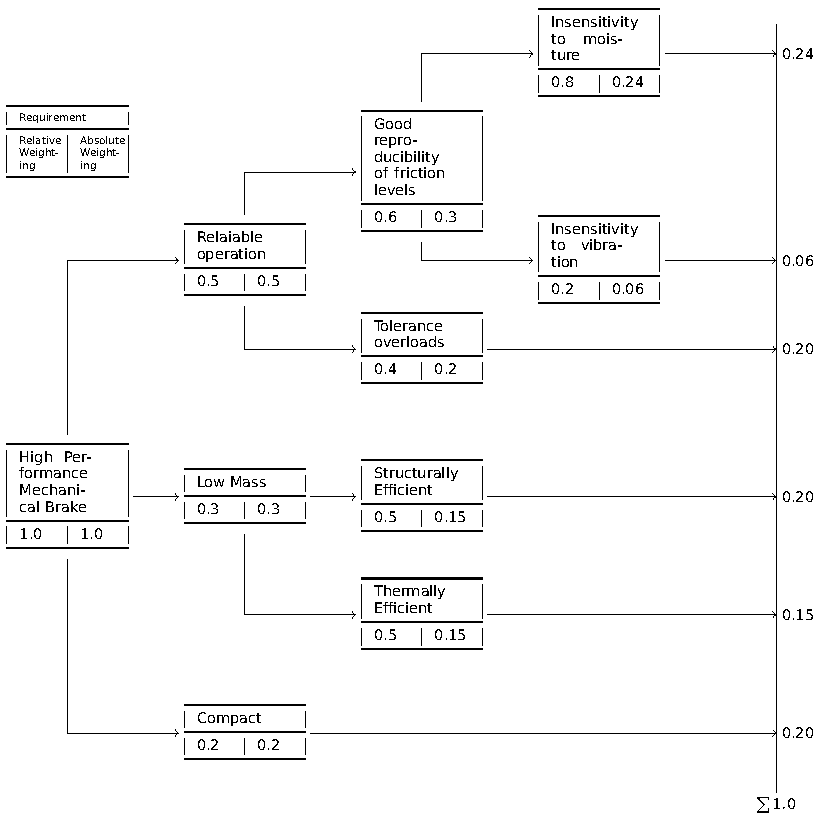
\includegraphics[width=0.25\textwidth]{figures/build/wot.pdf}
        \label{fig-wot}
      \end{tikzfigure}

      The Weighted Objectives Tree approach focuses on unpacking the design brief into lower-level requirements that can be assessed or measured through either quantitative and qualitative techniques (Figure~\ref{fig-wot}). Weighted Objectives Trees are particularly useful for highly-complex and inherently hierarchical products.

      \vspace{1em}

      The high-level objective is usually given a weighting of 1.0. This value of unity has to be split amongst the next level of objectives. Taking the example in Figure~\ref{fig-wot}, it was decided that reliability was more important than low-mass and compactness by a factor of 0.5 to 0.3 to 0.2.

      \vspace{1em}

      These relative weightings have to be multiplied by the value of the weighting in the next level up to get the absolute weightings. Since the objective at the next level up has a value of unity, the absolute weightings are still 0.5, 0.3 and 0.2. This process is followed down to all the root-objectives. 

      \vspace{1em}

      At any particular level the relative weightings always add up to 1.0. The absolute weightings get smaller and smaller as the tree goes down to lower levels. By definition, the sum of the absolute weightings of all the root objectives must come to exactly 1.0.
    }

    \column{0.5}

    \block[]{Multi-Criteria Decision Analysis}{

      \begin{tikzfigure}[MCDA comparing two potential projects]
        \centering
        \label{tbl-mcda}
        \small
        \begin{tabular}{l l l l l l}
        \toprule
        & & \multicolumn{2}{c}{\textbf{Project A}} & \multicolumn{2}{c}{\textbf{Project B}} \\
        \textbf{Criteria} & Weighting & Score & Weighted & Score & Weighted \\
        \midrule
        Compatibility with strategic objectives & 7
        & 4
        & 28
        & 4
        & 28 \\
        High Market Value
        & 9
        & 4
        & 36
        & 4
        & 36 \\
        Genuine advantages over competition
        & 9
        & 4
        & 36
        & 5
        & 45 \\
        Generate or save large amounts of money
        & 10
        & 4
        & 40
        & 4
        & 40 \\
        Contact with the market
        & 8
        & 4
        & 32
        & 4
        & 32 \\
        Technical expertise available
        & 4
        & 5
        & 20
        & 3
        & 12 \\
        Commercial expertise available
        & 7
        & 1
        & 7
        & 1
        & 7 \\
        Project management resources available
        & 4
        & 3
        & 12
        & 3
        & 12\\
        Clear route for implementation
        & 4
        & 2
        & 8
        & 2
        & 8 \\
        Evolving/lurking risk factors
        & 6
        & 2
        & 12
        & 2
        & 12 \\
        Compliance with industry standards
        & 3
        & 2
        & 6
        & 2
        & 6 \\
        Total 
        & 450
        & 44
        & 292
        & 46
        & 317 \\
        \midrule
        \% of Total & & 65\% & & 70\% \\
        Rank & & 2 & & 1 \\
        \bottomrule
        \end{tabular}
        \end{tikzfigure}

      MCDA is very similar to the controlled convergence strategy in that it is a matrix formed of rows denoting your requirements and columns denoting your concepts. However, instead of using a datum concept, each concept is scored separately against the criteria and is typically performed using a Likert scoring scale (Table~\ref{tbl-mcda}). Each requirement can also be weighted based on their priority/relative importance. The scores and weights are then summed to create an overall score for the concept. The concept with the greatest score is often considered the most suitable given the PDS, but it is always important to reflect and investigate whether certain features of the other concepts can be merged/combined to generate a further, more refined concept.

      \vspace{1em}
      
      \textbf{Pair-Wise Comparison} Applying weightings to the requirements can be a challenge but methods do exist to help us generate these weightings. Pair-wise comparison is one such method where you take each requirement and compare it with all the other requirements in your PDS. You then determine which requirement is more important for your design. Performing this across all your requirements forms a matrix of comparisons. These can be re-ordered to highlight the order of priority of your requirements. Taking the most important requirement as the highest weighted requirement, all the other requirements can then be scaled to match.

      \begin{tikzfigure}[Pair-wise comparison for weighting requirements]
        \centering
        \begin{tabular}{l l | l l l l l l l l l}
        \toprule
        \textbf{Function} & & A & B & C & D & E & F & G & H & I \\
        \midrule
        Functionality & A & - & A & C & D & A & F & A & AH & I \\
        Durability & B & - & - & C & D & B & B & B & H & BI \\
        Quality & C & - & - & - & D & C & F & C & H & C \\
        Affordability & D & - & - & - & - & D & F & D & D & I \\
        Manufacturability & E & - & - & - & - & - & F & E & H & E \\
        Usability & F & - & - & - & - & - & - & F & FH & I \\
        Maintainability & G & - & - & - & - & - & - & - & H & I \\
        Safety & H & - & - & - & - & - & - & - & - & I \\
        Marketability & I & - & - & - & - & - & - & - & - & - \\
        \bottomrule
        \end{tabular}
      \end{tikzfigure}

    }

    \block[]{Dot-Sticking}{
      \begin{tikzfigure}[Dot sticking]
        \centering
        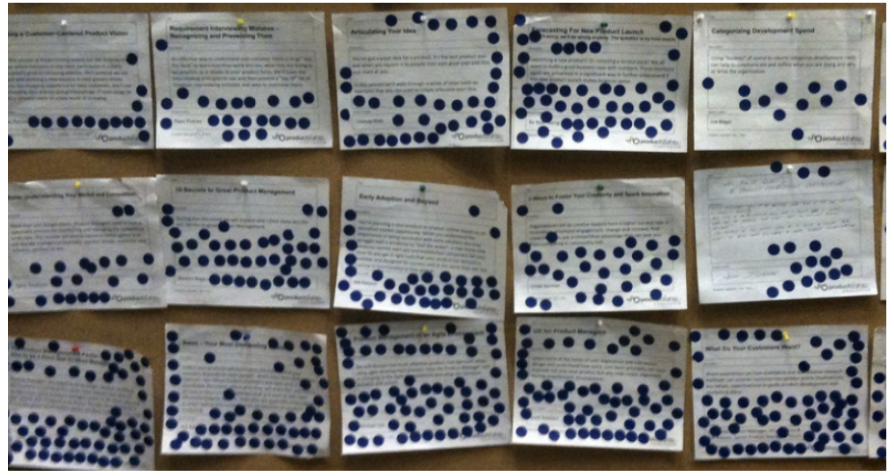
\includegraphics[width=0.3\textwidth]{figures/dot-sticking.png}
        \label{fig-dot}
      \end{tikzfigure}
      Dot sticking (Figure~\ref{fig-dot}) is the method of voting for your preferred concept to carry forward. The reviewers of the concepts are provided with sticky dots (on-line forms are increasingly used) and they are asked to place the dot on their preferred concept. Each concept should be presented in the same manner so as to avoid bias in the selection process.

      \vspace{1em}
      
      The technique is very simple and can be used to great effect when you need wider stakeholder engagement with the design process. In addition, it is very quick and can help reduce the number of concepts down to a small number in a short space of time. It is a very good tool to get initial feedback on the concepts you have generated.
    }
  
    \block[]{References}{
      \printbibliography[heading=none]{}
    }
  \end{columns}
  
  
  
  
  
  \end{document}